
\chapter{TFPM in two dimensions} % Main chapter title

\label{Chapter3} % For referencing the chapter elsewhere, use \ref{Chapter1} 

\lhead{Chapter 2. \emph{Parabolic and 2D Problem}}

\subsection{Convection-Diffusion-Reaction Problem}

\begin{align}
\mathbb{L}u & \equiv  -\epsilon^{2} \Delta u + p(\textbf{x})u_{x} + q(\textbf{x})u_{y} + b(\textbf{x})u = f(x), \forall \textbf{x} = (x,y) \in \Omega\\
u \large{|}_{\partial{\Omega}} & = 0
\end{align}

For the sake of simplicity, we assume that $\Omega = [0,1] \times [0,1]$ and we have a uniform mesh, i.e
$h = N^{-1}$ be the mesh size and 
\begin{align}
 x_{i} = ih, y_{j} = jh, 0 \leq i , j \leq N
\end{align}

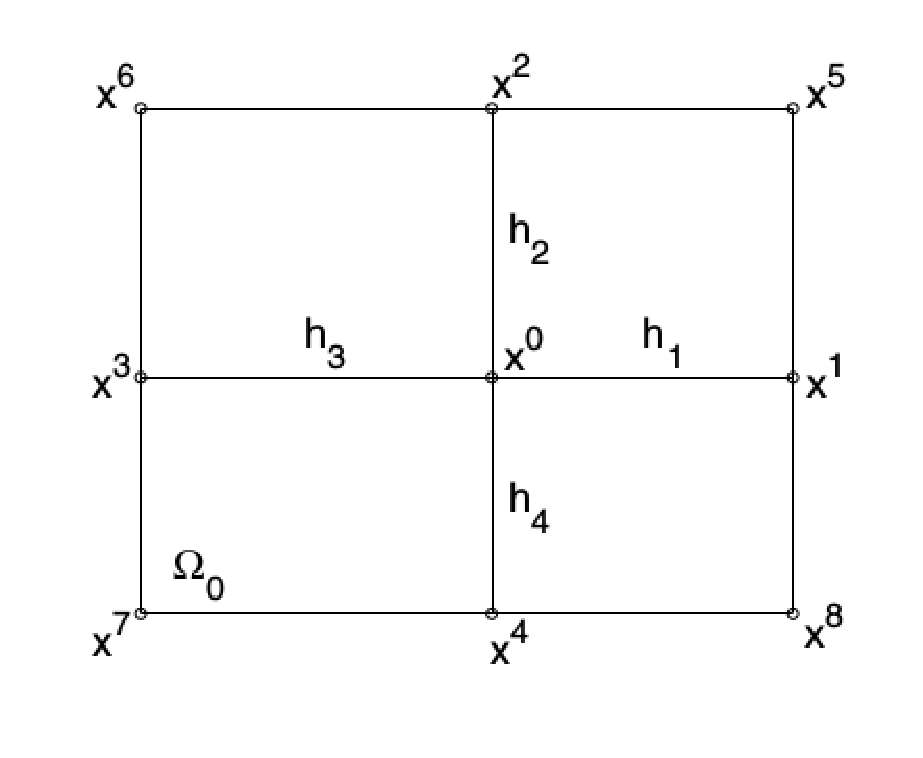
\includegraphics[width =8cm,height = 5cm]{Figures/cell_1.eps}

Then $\{ P_{i,j} = (x_i , y_j ), \hspace{0.3cm} 0 \leq i, j \leq N \}$ are the mesh points.
We construct our TFP scheme for (3.1) on the cell $\Omega_{0}$. We approximate the 
problem  on the cell as follows

\begin{align}
 -\epsilon^{2}\Delta+p_{0}(x)u_{x} + q_{0}u_{y} + b_{0}u = f_{0}
\end{align}
with $p_{0} = p(\textbf{x}^{0}),\hspace{1mm} q_{0} = q(\textbf{x}^{0}),\hspace{1mm} b_{0} = b(\textbf{x}^{0}),\hspace{1mm} f_{0} = f(\textbf{x}^{0})$\\

We consider the case $ b_{0}>0$

Let
\begin{align}
 u(x,y) = \frac{f_{0}}{b_{0}} + v(x,y)\text{exp} \Bigg{(}\frac{p_{0}x + q_{0}y}{2 \epsilon^2}\Bigg{)}
\end{align}
Then we have,

\begin{align}
 -\epsilon^{2} \Delta{v} + d^{2}_{0} = 0
\end{align}

with $d^{2}_{0} = b_{0} + \frac{p_{0}^{2}+q_{0}^{2}}{4 \epsilon^2} $\\
Let $\mu_{0} = d_{0}/\epsilon$, and

\begin{align*}
 H_{4} = \bigg{\{} v(x,y)|\hspace{2mm}v =  c_{1}e^{-\mu_{0}x} + c_{2}e^{\mu_{0}x} + c_{3}e^{-\mu_{0}y} + c_{4}e^{-\mu_{0}y},\hspace{3mm} \forall c_{i} \in \mathbb{R} \bigg{\}}
\end{align*}
Then we take the scheme as

\begin{align}
 \alpha_{1}V_{1} + \alpha_{2}V_{2} + \alpha_{3}V_{3} + \alpha_{4}V_{4} + \alpha_{0}V_{0} = 0
\end{align}
with $V_{j} = v(\textbf{x}^{j})$. Thus we obtain
\begin{align}
 \alpha_{1}e^{-\mu_{0}h} + \alpha_{2} + \alpha_{3}e^{\mu_{0}h} + \alpha_{4}+\alpha_{0} &= 0\\
 \alpha_{1}e^{\mu_{0}h} + \alpha_{2} + \alpha_{3}e^{-\mu_{0}h} + \alpha_{4}+\alpha_{0}&= 0\\
 \alpha_{1} + \alpha_{2}e^{-\mu_{0}h} + \alpha_{3} + \alpha_{4}e^{\mu_{0}h}+\alpha_{0}&= 0\\
 \alpha_{1} + \alpha_{2}e^{\mu_{0}h} + \alpha_{3} + \alpha_{4}e^{-\mu_{0}h}+\alpha_{0} &= 0
\end{align}
For any constant $\alpha_{0} \in \mathbb{R}$ the system (1.10) to (1.13) has the unique solution

\begin{align}
 \alpha_{1} = \alpha_{2} = \alpha_{3} = \alpha_{4} = \frac{-\alpha_{0} }{e^{\mu_{0}h}+e^{-\mu_{0}h}+2} \equiv \frac{-\alpha_{0}}{4\cosh^2\bigg{(}\frac{\mu_{0}h}{2}\bigg{)}}     
\end{align}

On taking

\begin{align}
 \alpha_{0} = \frac{e^{\mu_{0}h}+e^{-\mu_{0}h}+2}{e^{\mu_{0}h}+e^{-\mu_{0}h}-2} \equiv \frac{\cosh^2\bigg{(}\frac{\mu_{0}h}{2}\bigg{)}}{\sinh^2\bigg{(}\frac{\mu_{0}h}{2}\bigg{)}}
\end{align}

we have

\begin{align}
 \alpha_{1} = \alpha_{2}=\alpha_{3} = \alpha_{4} = -\frac{1}{e^{\mu_{0}h}+e^{-\mu_{0}h}+2} \equiv - \frac{1}{4 sinh^{2}\bigg{(}\frac{\mu_{0}h}{2}\bigg{)}}
\end{align}

We ultimately get the following scheme
\begin{align}
 \begin{split}
  U_{0} -& \frac{e^{-\frac{p_{0}h}{2\epsilon^2}}U_{1}+e^{-\frac{q_{0}h}{2\epsilon^2}}U_{2}+e^{\frac{p_{0}h}{2\epsilon^2}}U_{3}+e^{\frac{q_{0}h}{2\epsilon^2}}U_{4}}
  {4cosh^2\bigg{(}\frac{\mu_{0}h}{2}\bigg{)}}\\
  =& \frac{f_{0}}{b_{0}}\Bigg{(}1-\frac{e^{-\frac{p_{0}h}{2\epsilon^2}}+e^{-\frac{q_{0}h}{2\epsilon^2}}+e^{\frac{p_{0}h}{2\epsilon^2}}+e^{\frac{q_{0}h}{2\epsilon^2}}}
  {4cosh^2\bigg{(}\frac{\mu_{0}h}{2}\bigg{)}}\Bigg{)}
 \end{split}
\end{align}
with
\begin{align}
U_{j} = u(\textbf{x}^{j}) = \frac{f_{0}}{b_{0}} + V_{j}\text{exp}\Bigg{(} \frac{p_{0}x + q_{0}y}{2 \epsilon ^2} \Bigg{)}
\end{align}

\subsection{Example}
Consider the following convection-diffusiion-reaction problem along with the given conditions
\begin{align}
 -\epsilon^{2}\Delta u &+ p(\textbf{x})u_{x} + q(\textbf{x})+u_{y}+b(\textbf{x})u = f(\textbf{x}),\hspace{0.5cm} \forall x = (x,y) \in \Omega\\
 u|_{\partial{\Omega}} &= 0
\end{align}
where
\begin{align*}
 &\Omega = [0,1]^2,\hspace{2mm} p(\textbf{x}) = 1,\hspace{2mm} q(\textbf{x}=0),\hspace{2mm} b(\textbf{x}) = 1,\\
 &f(x,y) = [2\epsilon^2 + y(1-y)]\bigg{[}e^{\frac{x-1}{\epsilon^2}} + (x-1)e^{-\frac{1}{\epsilon^2}-x} -x\bigg{]} + y(1-y)\big{(}e^{-\frac{1}{\epsilon^2}}-1\big{)}
\end{align*}
The exact solution of the problem is given by
\begin{align*}
 u(x,y) = y(1-y)\bigg{[}e^{\frac{x-1}{\epsilon^2}} + (x-1)e^{-\frac{1}{\epsilon^2}} -x \bigg{]} 
\end{align*}

The following plots and error estimates have been obtained on solving the above example using the 
tailored finite point method.
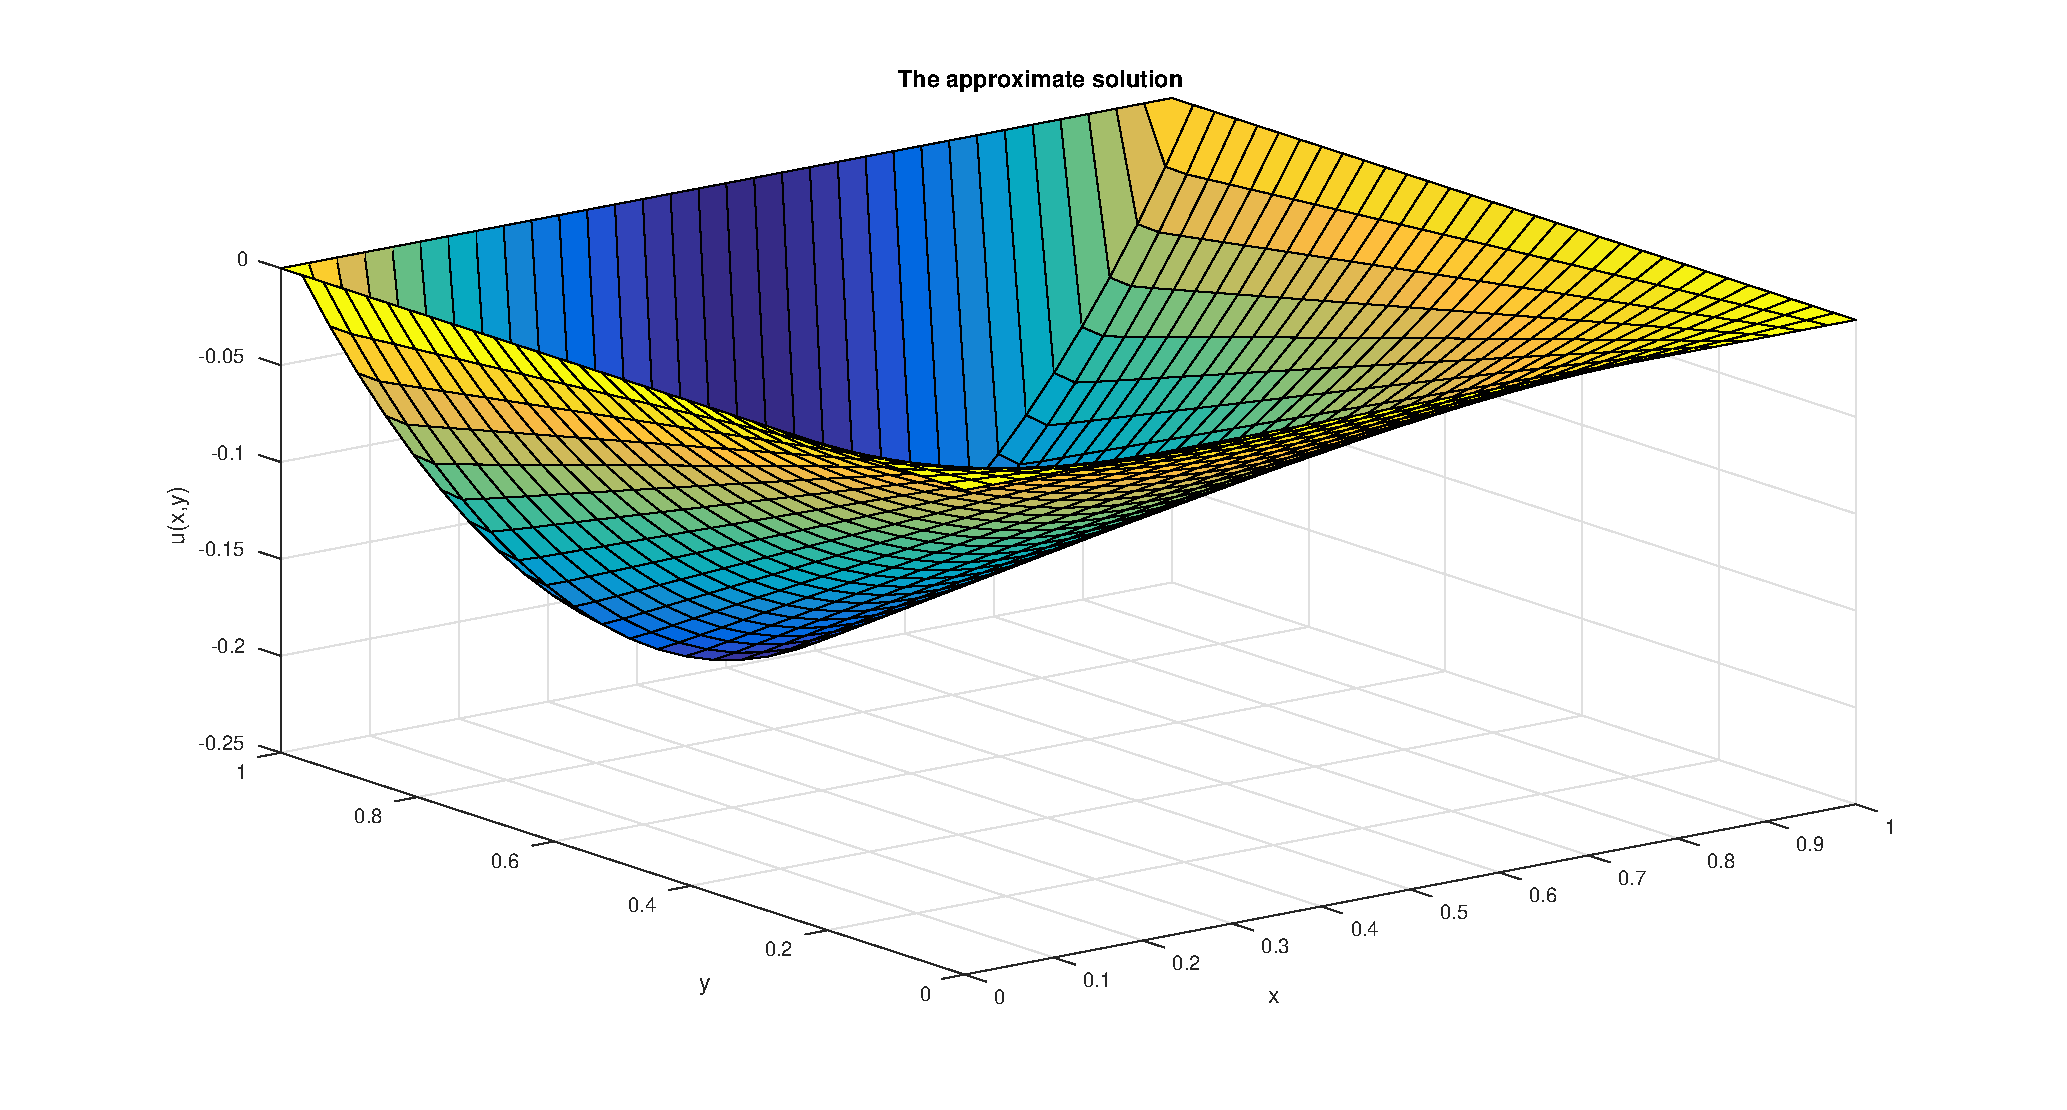
\includegraphics[height=8cm]{Figures/CDR_approx_2.eps}\\
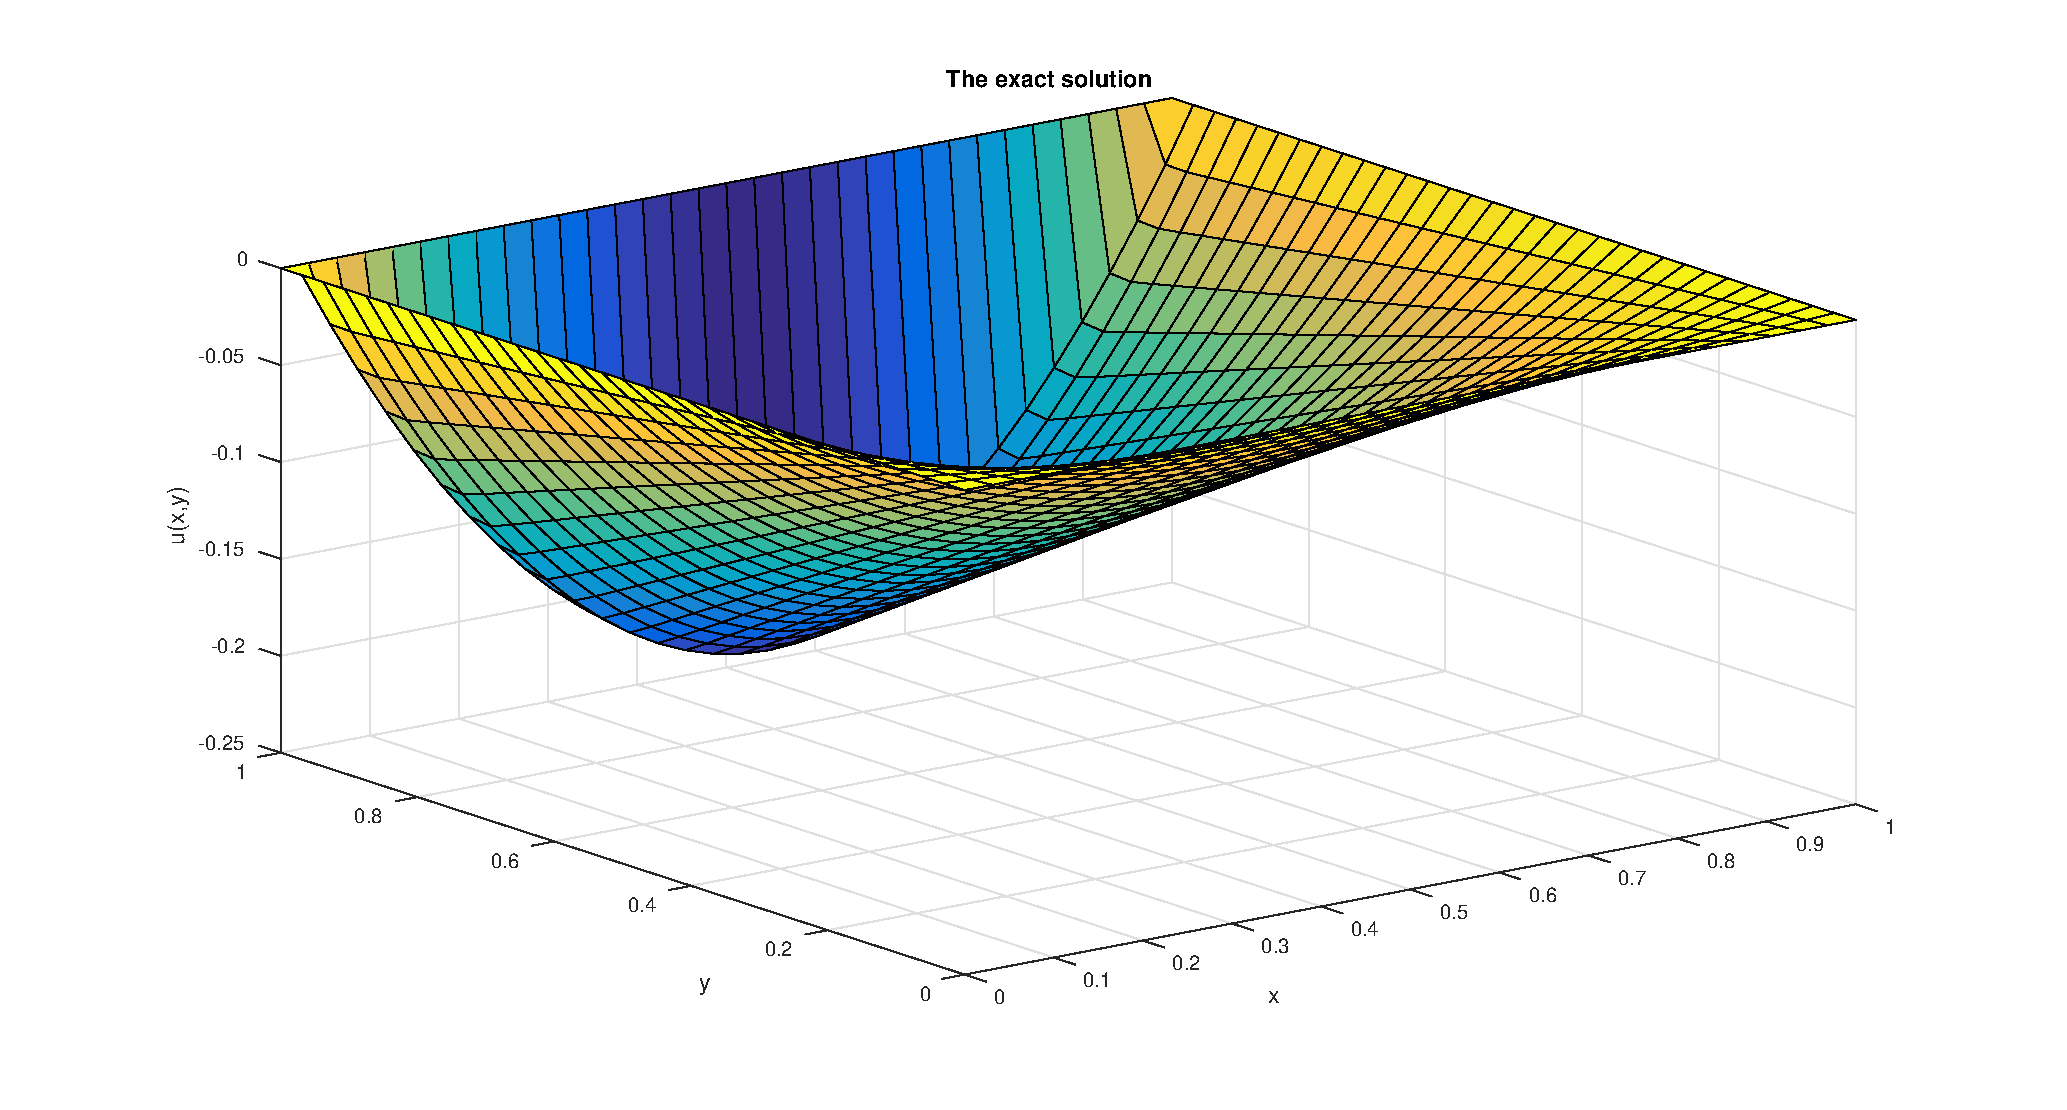
\includegraphics[height=8cm]{Figures/CDR_exact_1.eps}\\

\begin{tabular}{|c|c|c|c|c|c|}
   \hline
  & mesh size h  & 1/16  & 1/32 & 1/64 &  1/128\\
  \hline
 $\epsilon = 0.1$ & Error  & 0.0082  & 0.0032 & 9.4071e-04 &  2.2276e-04\\
 \hline
   &Order & -  &  1.3576  & 1.7662 & 2.0783\\
\hline
  $\epsilon = 0.05$ & Error  & 0.0061  & 0.0038 & 0.0021 &  8.400e-04\\
 \hline
   &Order & -  &  0.6828 & 0.8556 & 1.32\\
\hline
  $\epsilon = 0.01$ & Error  & 0.0048  & 0.0025 & 0.0013 &  6.7100e-04\\
 \hline
   &Order & -  &  0.9411  & 0.9434 & 0.9541\\
\hline
\end{tabular}

